\chapter{Технологический раздел}
\section{Выбор средств разработки}
\subsection{Выбор целевой платформы}
Программный продукт поиска аномалий не затачивается под работу на конкретной ОС. Его корректная работа протестирована на ОС Windows и OS Linux Данный выбор обусловлен широкой распространенностью ОС Windows и Linux, большим количеством средств разработки для данных платформ, что дает возможность выбирать
язык программирования и сопутствующие инструменты, ориентируясь на возможность простого и надежного решения рассматриваемой
задачи, а не на ограничения целевой платформы.

Программный комплекс для сбора данных разрабатывается для OS Linux, в силу особенностей функционирования графического редактора, плагин для которого входит в состав этого программного комлекса.
\subsection{Выбор языка программирования}
Для написания программы поиска аномалий используется язык C++, так
как с версии С++11 он сочетает в себе возможности функционального и
объектно-ориентированного подходов.
С помощью функционального подхода удобно описывать алгоритмы
и математические выражения, необходимые для решения поставленной
задачи. Использование функциональных средств существенно упрощает
описание операций над последовательностями входных данных.
В то же время, применение объектно-ориентированных подхода дает
возможность проектирования приложения в терминах объектов предметной
области и их поведения, что позволяет контролировать сложность
программы, предлагать наглядные и емкие абстракции и четко выделять
сферы ответственности программных модулей.
Также объектно-ориентированные языки позволяют построение приложения с графическим интерфейсом пользователя с учетом известных рекомендаций и правил.
Дополнительным преимуществом языка C++ является большая база
документации по самому языку и стандартным библиотекам.


В качестве языка написания плагина к графическому редактору был выбран язык С++ в силу того, что сам редактор поддерживает только плагины на этом языка. 
Для написания бекенд-сервера был выбран язык Golang вместе с библиотекой  mgo для доступа к базе данных . Плюсы этого языка:
\begin{enumerate}
	
	\item Скорость разработки	 	
	
	\item Производительность
	
	\item Удобная реализация легковесных потоков 
\end{enumerate}

Для предварительной обработки данных использовался языка bash. Bash - это мощный и простой в использовании язык сценариев. Он позволяет 	 легко перемещать курсор и редактировать текст команды в командной строке, поддерживает историю команд: дает возможность повторить или при необходимости изменить команду, которая была введена в командной строке ранее. Позволяет легко указать команде, откуда брать входные данные и куда направлять выходные данные. Поддерживаются псевдонимы - создание кратких обозначения для однострочных команд.

\subsection{Выбор среды разработки и отладки}
Из-за использования сразу нескольких языков, в процессе работы над программным комплексом, было использовано несколько сред разработки.
Qt Creator - современная кросс-платформенная среда разрабтки, которая предоставляет широкие возможности разработки программ на С++, а так же их отладки. Qt Creator так же поддерживает работу со сторонними плагинами, что позволило использовать плагин работы с системой контроля версий.

Для работы с языком Golang был использован текстовый редактор Visual Studio Code с набором плагином для языка Golang. Набор плагинов к текстовому редактору позволяет осуществлять запуск и отладку кода прямо из редактора, а так же позволяет осуществлять автоматическое форматирование кода.

Для работы с bash использовался nano - консольный текстовый редактор для Unix и Unix-подобных операционных систем, основанный на библиотеке curses. В настоящее время включен в дистрибутивы Ubuntu по умолчанию и в установке не нуждается.
\section{Выбор базы данных}
Для сохранения элементов данных была выбрана документо-ориентированная база данных MongoDb. Основные преимущества MongoDb:
\begin{itemize}
	\item Отсуствие четкой структуры хранения данных
	\item Возможность выгружать и загружать файлы в JSON-формате.
	\item Быстрая вставка элементов
	\item Быстрое извлечение простых данных
\end{itemize}
\section{Система контроля версий}
В процессе разработки программы использовалась система контроля
версий Git.
Система контроля версий позволяет вносить в проект атомарные
изменения, направленные на решения каких-либо задач. В случае
обнаружения ошибок или изменения требований, внесенные изменения
можно отменить.
Кроме того, с помощью системы контроля версий решается вопрос
резервного копирования.
Особенности Git:
\begin{itemize}
\item Предоставляет широкие возможности для управления изменениями
	проекта и просмотра истории изменений
 \item Данная система контроля версий является децентрализованной, что
позволяет иметь несколько независимых резервных копий проекта.
\item Поддерживается хостингом репозиториев GitHub и Gitlab.
\item Поддерживается средой разработки Qt Creator и Visual Studio Code.
\end{itemize}
\section{Библиотека Galgo}
Для подбора параметров алгоритмов была использована библиотека GALGO версии 2. Она позволяет не вдаваясь в нюансы работы гентических алгоритмов, подобрать необходимые значения параметров алогритмов. В качестве функции, необходимой для работы генетического алгоритма, использовался алгоритм поиска аномалий. В качестве выходного значения функции использовался AUC ROC.
\section{Формат файлов}
На вход программе поиска аномалий подается файл следующего формата: одна строка содержит  в ненормализованном виде  атрибуты данных одого элемента.
\begin{lstlisting}[language=c++,,escapeinside={(@}{@)},caption={Пример входного файла программы поиска аномалий}] 
9 10 23 4
1 3  2  1
1 4  9  12
6 7  4  44
\end{lstlisting}
Для проверки корректности алгоритма использовался иной формат входных файлов. Одна строка содержит в нормализованном виде n-1 атрибутов одного элемента, на n-ой позиции в строке расположена метка аномальноси объекта('yes' или 'no'). Атрибуты элементов разделяются запятной.


Для проверки корректности алгоритма использовался иной формат входных файлов. Одна строка содержит в нормализованном виде n-1 атрибутов одного элемента, на n-ой позиции в строке расположена метка аномальноси объекта('yes' или 'no'). Атрибуты элементов разделяются запятной.
\begin{lstlisting}[language=c++,,escapeinside={(@}{@)},caption={Пример входного файла программы поиска аномалий для проверки корректности алгоритма}] 
0.467651,0.321584,0.76888,0.24663,0.838799,0.099737,0.29834,1.0,'no'
0.496412,0.220491,0.77603,0.36598,0.91993,0.08914,0.279479,2.0,'no'
0.519133,0.404464,0.76012,0.33498,0.80122,0.09239,0.271238,3.0,'no'
0.19965,0.547373,0.374284,0.362223,0.817017,0.0,0.177913,4.0,'yes'
0.847261,0.286361,0.0,0.217792,0.0,0.019135,1.0,5.0,'no'
\end{lstlisting}
Третий формат возможный формат файлов предназначен для демонстрационного режима работы программы. В начале строки располагается текстовое описание элемента(без пробелов), следующие два атрибута характеризуют элемент в двумерном пространстве.
\begin{lstlisting}[language=c++,,escapeinside={(@}{@)},caption={Пример входного файла программы поиска аномалий демонстрационного режима}] 
edit 23 53
undo 35 547
redo 100 0
editcut 46 3
\end{lstlisting}

\section{Библиотека KUserFeedback}

В качестве вспомогательной библиотеки для сбора стастики используется библиотека KUserFeedback компании KDAB. Эта библиотека включает в себя С++ Qt клиентскую часть, а так же сервер, написанный на PHP. Их сервер  и значительная часть функций не требуется, будет использоваться только часть собирающую телеметрию. KUserFeedBack позволяет  собрать библиотеку по частям и линковать к нашему приложению только необхоимые модули. В программе используется модуль Core. Модуль Core содержит абстракный класс источника данных, от которого можно наследовать различные источники данных.

\section{Установка программного обеспечения}

У программы поиска аномалий нет зависимостей от внешних служб и программ, установленных в операционной системе, а также отсутствует
необходимость в модификации системных и пользовательских настроек, поэтому было принято решение не разрабатывать инсталлятор.
Исполняемым файлом программы является mainProject.exe(windows) или mainProject(linux).

Программа для сбора данных требует установленного графического редактора Krita с плагином  телеметрии.
Исполняемым файлом бекенд-сервера является файл server.
\section{Пример работы программы}
\begin{figure}[!h]
	\centering
	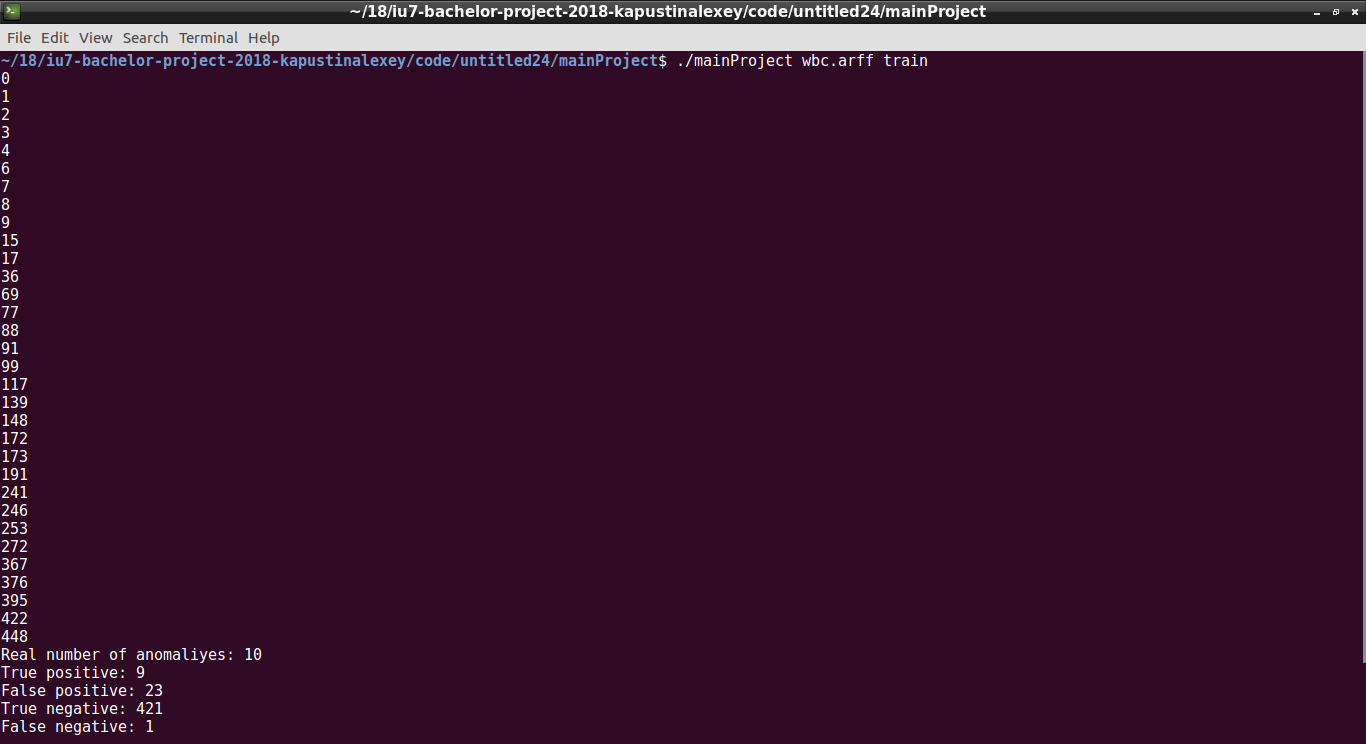
\includegraphics[width=.8\textwidth]{img/screenPr.png}
	\caption{Пример работы программы для набора данных wbc}
	\label{fig10}
\end{figure}
Приведен пример работы программы на операционной системе Lubuntu 16.04(Linux). Имя программы - mainProject, первый аргумент - обрабатываемый файл, второй аргумент - режим работы. В результате работы программы можно увидеть список найденных аномалий, а так же количество правильно или неверно классифицировашихся элементов.
\section{Использование программы для поиска аномалий}
Запуск программы осуществляется из командной строки. Первыйм аргументом
нужно передать имя файла для анализа. Вторым передается режим работы программы.Существуют 3 основых режима работы программы:
\begin{itemize}
	\item Проверочный. Запуск этого режима осуществлятся при помощи передачи в качестве второго параметра слова "train"\ .
	Этот режим обрабатывает размеченные наборы данных(данные должны быть предоставлены в описанном выше формате). В результе работы программы на экран выводится список полученных аномалий, метрики полноты, точности, площади по графиком РОК-кривой, количество истинно позитивных, истинно негативных, ложно негативных, ложно позитивных элементов данных.
	\item Основной. Для запуска этого режима нужно либо не указывать второй параметр, либо указать его некорректно(не "train"\ или "demo"\ ). Этот режим обрабатывает неразмеченные наборы данных(в описанном выше формате). В результате работы  программы выводится список обнаруженный аномалий.
	\item Демонстрационный. Для запуска нужно передать второй аргумент равный "demo"\ . Предназначен наглядного представления результатов поиска аномалий в двумерном пространстве. Режим обрабатывает неразмечнные наборы данных. 
\end{itemize}
